\documentclass{beamer}

\usepackage[utf8]{inputenc}
\usepackage[T1]{fontenc}
\usepackage[ruled,vlined,linesnumbered]{algorithm2e}
\usepackage{tikz}

\usepackage{verbatim}
\usetikzlibrary{arrows,shapes}

\SetAlFnt{\small}
\SetAlCapFnt{\large}
\SetAlCapNameFnt{\large}

%%% algorithm2e environment with "Algoritmi"-caption.
\newenvironment{finalgo}[1][htb]{
  \renewcommand{\algorithmcfname}{Algoritmi}
  \begin{algorithm}[#1]
}{\end{algorithm}}

%%% To be able to not numbering individual lines:
\let\oldnl\nl% Store \nl in \oldnl
\newcommand{\nonl}{\renewcommand{\nl}{\let\nl\oldnl}}

%%% argmin
\DeclareMathOperator*{\argmin}{arg\, min}

\title{{\rmfamily\scshape Lyhimpien polkujen hakualgoritmit ja -järjestelmät}}
\author{$\mathfrak{Rodion \, Efremov}$}
\date{}
\institute{Tietojenkäsittelytieteen laitos, Helsingin yliopisto}

\usetheme{Ilmenau}
\usecolortheme{beaver}
\usefonttheme[onlymath]{serif}

\begin{document}
\maketitle
% Declare layers
\pgfdeclarelayer{background}
\pgfsetlayers{background,main}

%%% BEGIN: Määritelmät
\begin{frame}
\frametitle{Verkot}
\begin{itemize}
\item Suunnattu verkko on $G = (V, A)$, missä $V$ on solmujen joukko ja $A \subset V \times V$ on suunnattujen kaarien joukko.

\item Suuntaamaton verkko $G = (V, E)$ voidaan aina simuloida suunnatulla verkolla $(V, A)$ laittamalla $A$:han kaaret $(u, v)$ ja $(v, u)$ jokaisella suuntaamattomalla kaarella $\{u, v\} \in E$.

\item Jatkossa merkitsemme $n = |V|$ ja $m = |E|$.
\end{itemize}
\end{frame}
%%% END: Määritelmät

%%% BEGIN: BFS
\begin{frame}
\frametitle{Leveyssuuntainen haku}
\begin{itemize}
\item Toteutus vaatii vain jonon ja hajautustaulun.
\item Toimii ajassa $\mathcal{O}(n + m) \approx \sum_{i = 0}^N d_i$, missä $N$ on lyhimmän polun solmujen määrä ja $d$ keskiarvoinen solmun aste.
\end{itemize}
\end{frame}
%%% END: BFS

%%% BEGIN: BFS pseudocode
\begin{frame}
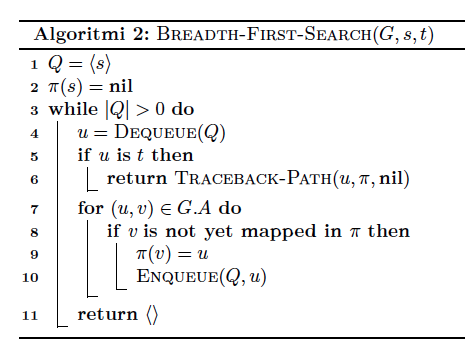
\includegraphics[width=\textwidth,keepaspectratio]{bfs}
\end{frame}
%%% END: BFS pseudocode

%%% BEGIN: BFS EXAMPLE
\begin{frame}
\tikzstyle{vertex}=[circle,fill=black!25,minimum size=20pt,inner sep=0pt]
\tikzstyle{selected vertex} = [vertex, fill=red!24]
\tikzstyle{edge} = [draw,thick,-]
\tikzstyle{weight} = [font=\small]
\tikzstyle{selected edge} = [draw,line width=5pt,-,red!50]
\tikzstyle{ignored edge} = [draw,line width=5pt,-,black!20]

\begin{figure}
\begin{tikzpicture}[scale=1.8, auto,swap]
    % Draw a 7,11 network
    % First we draw the vertices
    \foreach \pos/\name/\lbl in {{(0,2)/a/0}, {(2,1)/b/1}, {(4,1)/c/2},
                            {(0,0)/d/11}, {(3,0)/e/2}, {(2,-1)/f/2}, {(4,-1)/g/3}}
        \node[vertex] (\name) at \pos {$\lbl$};
    % Connect vertices with edges and draw weights
    \foreach \source/ \dest in {b/a, c/b, d/a, d/b,
                                         e/b, e/c, e/d,
                                         f/d, f/e,
                                         g/e, g/f}
        \path[edge] (\source) -- node[weight] {} (\dest);
    % Start animating the vertex and edge selection. 
    \foreach \vertex / \fr / \lbl in {d/1/1,a/2/0,f/3/2,b/4/1,e/5/2,c/6/2,g/7/3}
        \path<\fr-> node[selected vertex] at (\vertex) {\lbl};
    % For convenience we use a background layer to highlight edges
    % This way we don't have to worry about the highlighting covering
    % weight labels. 
    \begin{pgfonlayer}{background}
        \pause
        \foreach \source / \dest in {d/a,d/f,a/b,b/e,e/c,e/g}
            \path<+->[selected edge] (\source.center) -- (\dest.center);
        \foreach \source / \dest / \fr in {d/b/4,d/e/5,e/f/5,b/c/6,f/g/7}
            \path<\fr->[ignored edge] (\source.center) -- (\dest.center);
    \end{pgfonlayer}
\end{tikzpicture}
\end{figure}
\end{frame}
%%% END: BFS EXAMPLE

\end{document}